\documentclass[../main.tex]{subfiles}
\graphicspath{{\subfix{../images/}}}
\begin{document}

\chapter{Introduction}
\subfile{Introduction_Nutr.tex}

\chapter{Anatomy and Physiology of Nutrition}
\subfile{Anatomy_Nutr.tex}

\chapter{Nutrition}
\subfile{Nutrition.tex} % SI

\chapter{The Energy Requirements of Humans} % SI
\subfile{EnergyReq.tex}

\chapter{The Healthy Body Weight} %SI
\subfile{HealthyBodyWeight.tex}

\chapter{Basic Building Blocks of our Nutrition}
\subfile{BuildingBlocksFood.tex} %SI

\chapter{A Healthy Diet}

\subfile{HealthyDiet.tex} %SI A

\chapter{Glycemic Index (GLYX)}\label{chap:carbs}

\subfile{Glyx.tex}

\chapter{Glycemic Load}

\subfile{GlycemicLoad.tex}

\chapter{Tips for a Healthy Nutrition}

\subfile{TipsNutrition.tex}

\chapter{Special Foods and Drinks}\label{SpecialFoods} 

\subfile{SpecialFood.tex}
% Coffee -> talk about Espresso

\chapter{Risk and Troubles of Malnutrition}

\section{Problems of the Acid Base Balance}

\subfile{Malnutrition.tex} %eigentlich saure base

\section{Diabetes Type 2 --- a Disorder of the Metabolism}

\subfile{DiabetesType2.tex}

\chapter{Stress and Nutrition}

\subfile{StressNutrition.tex}

\chapter{Special Diets}

\subfile{SpecialDiets.tex}

\chapter{Annex Nutrition}

\subfile{AnnexNutrition.tex}

\chapter{55 Tips for a Conscious Approach to Nutrition}

\subfile{TipNutrition.tex}

\chapter{Recommended Literature}

\subfile{Lit_Nutrition.tex}

\chapter{Nutrition Test}

\subfile{NutrtitionTest.tex}

\chapter{Summary}

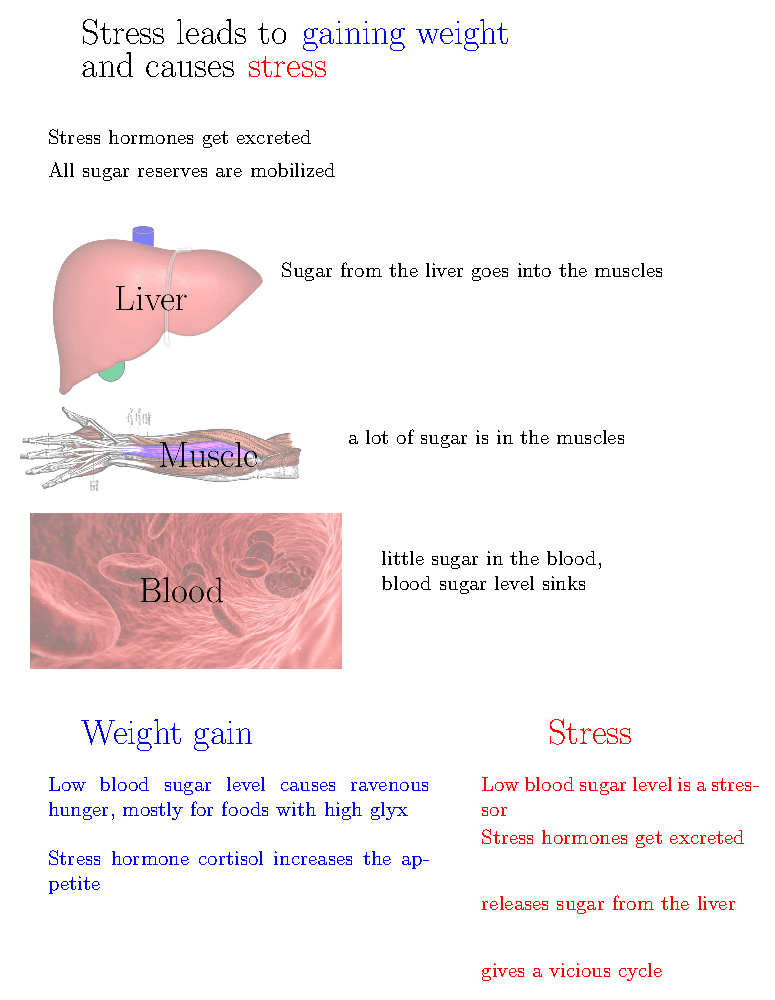
\includegraphics[width=\linewidth]{StressCauses}

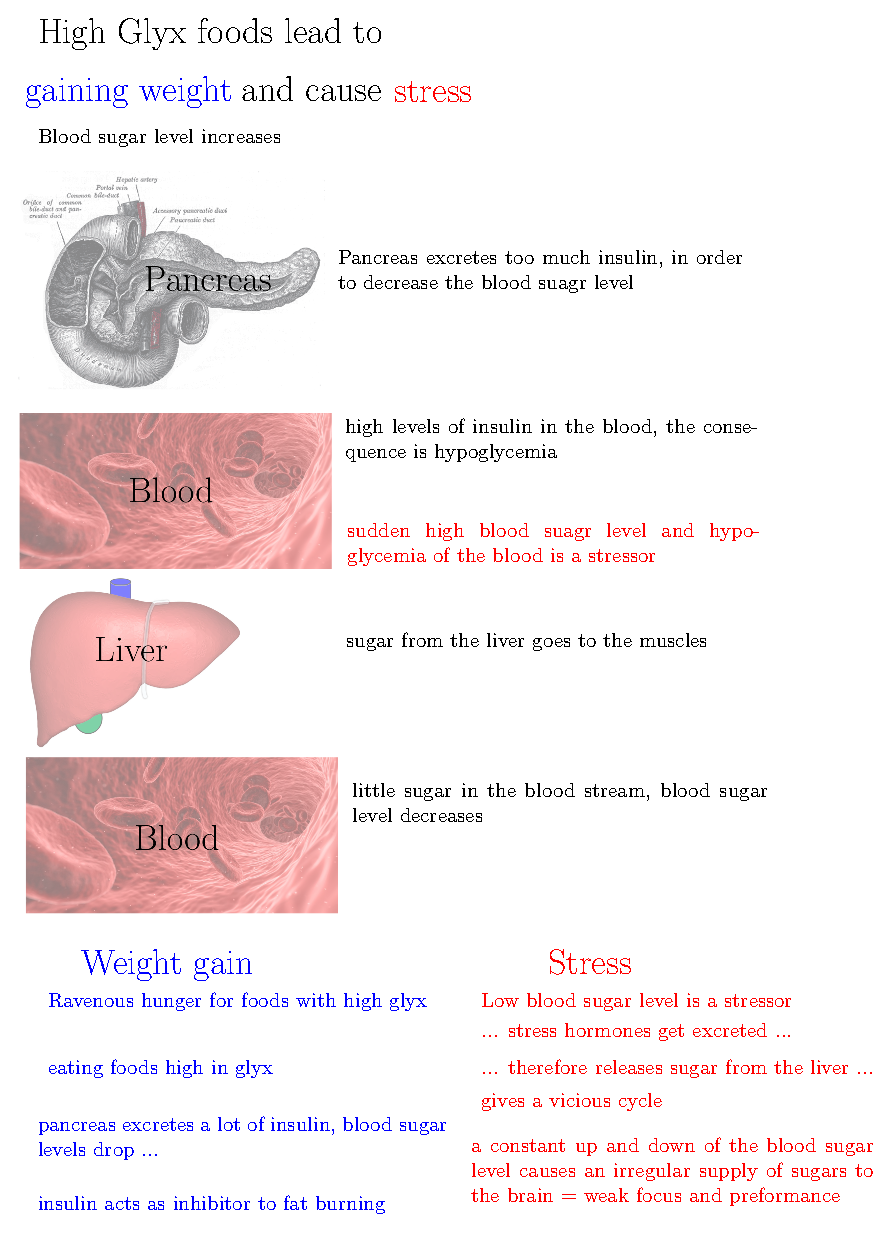
\includegraphics[width=\linewidth]{GlyxCauses}

Picture liver \cite{LiverPic}, \cite{MusclePic}, \cite{BloodPic}, \cite{PancreasPic}

\chapter{Practice Your Knowledge}

\subfile{Questions_Nutrition.tex}

% Food pyramid, explanaiton

% Maybe about gut flora, microbiome, cells in colon,
% General note of caution, need to know and find for yourself, many different diets out there

%Artificial sweetener --> not good, except polydiols (sugar, research) diabetes, overweight, even stevia, influence gut biome


% mushrooms, adaptogenics

%Different opinions, very complicated, follow your gut feeling
%Gluten - some say bad (show) some not
% Urdinkel, pure spelt, original spelt
%Soy antinutrient \label{FoodSoy} --> SpecialDiets.tex

\end{document}
